% !TeX root=debugging.tex

\section{Types of bugs}

\begin{frame}
    \frametitle{Types of bugs}
    \begin{figure}
        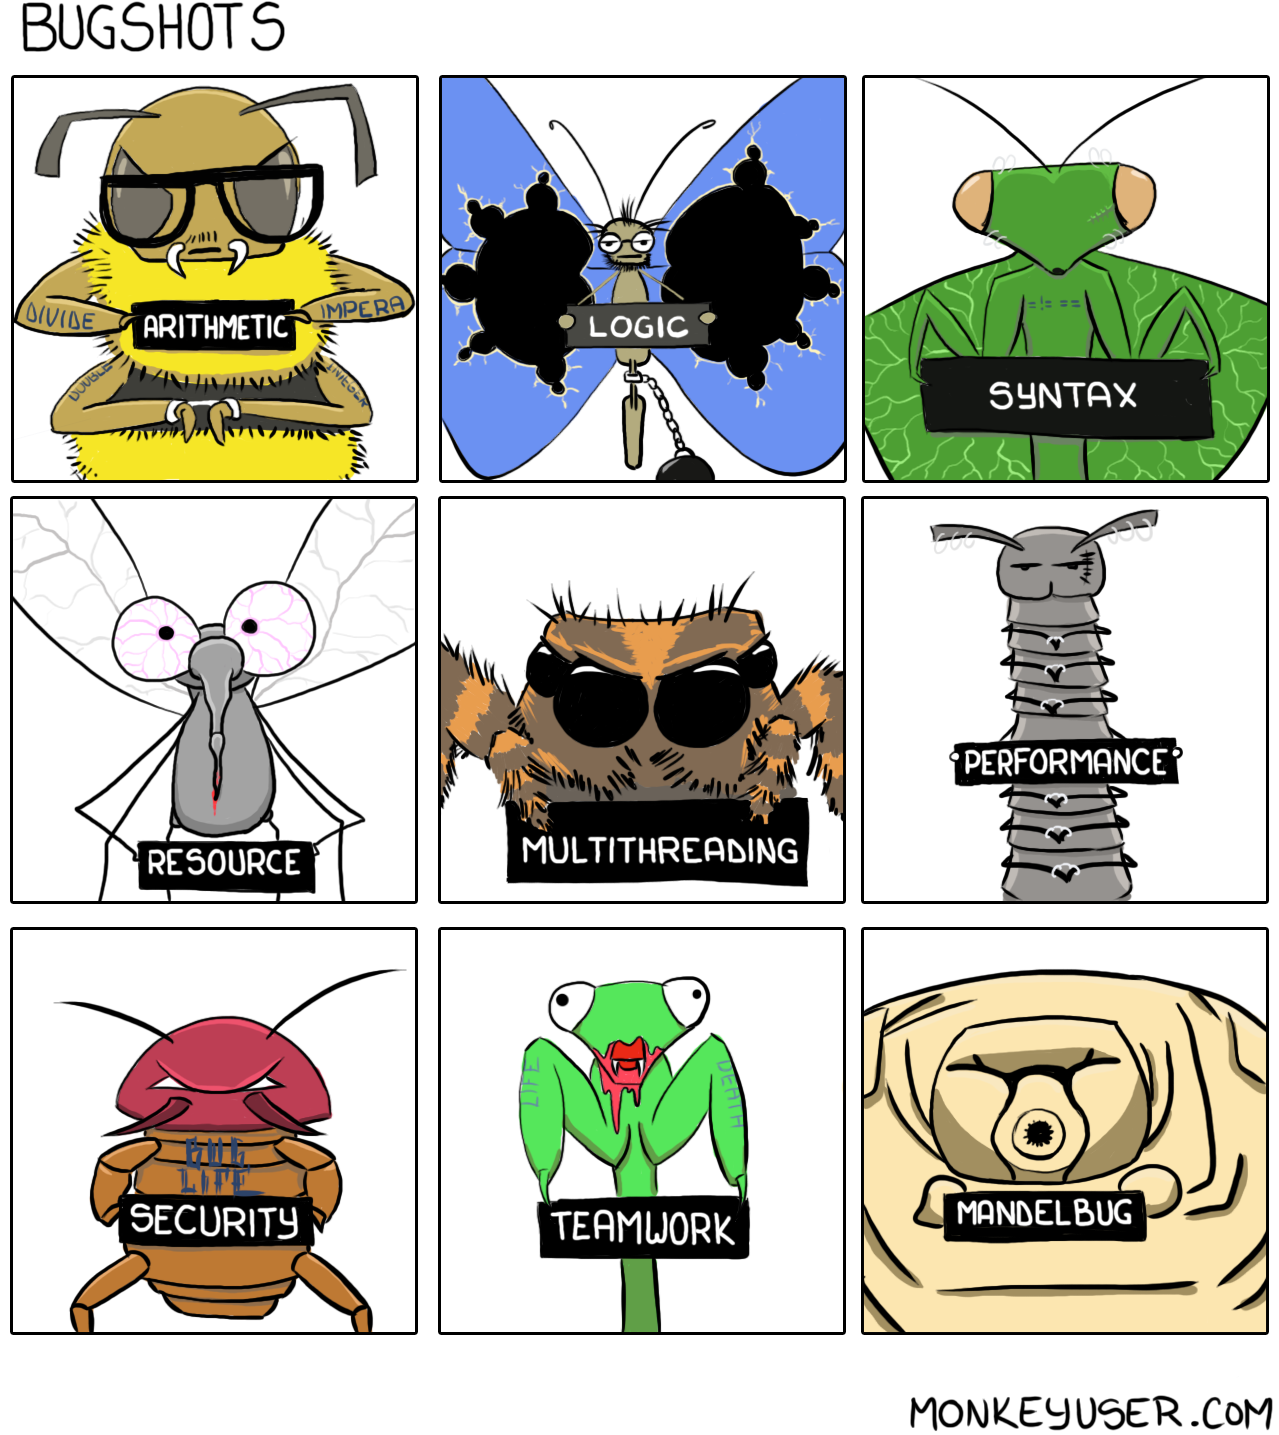
\includegraphics[height=0.8\textheight]{bugshots.png}
    \end{figure}
\end{frame}

\begin{frame}
    \frametitle{Types of bugs}
    \tikz[overlay]\node[rotate=-6] at (60ex,6ex) {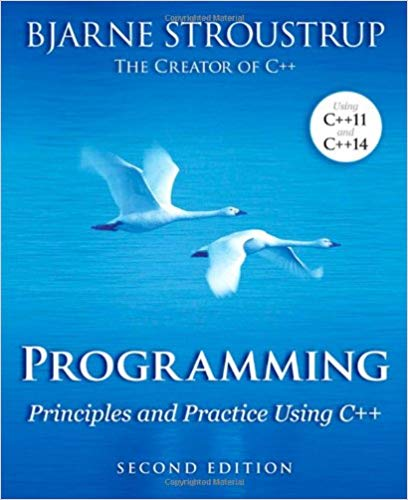
\includegraphics[width=0.3\textwidth]{Stroustrup_PPP.jpg}};
    \tikz[overlay]\node[rotate=-6] at (57ex,-9ex) {\footnotesize Chapter 5: Errors};
    \begin{itemize}[<+->]
        \item Compile-time errors
        \item Run-time errors
        \item Logic errors
    \end{itemize}
\end{frame}

\subsection<beamer:0>{Compile-time errors}

\begin{frame}<beamer:0>[fragile]
    \frametitle{Compile-time errors}
    \tikz[overlay]\node[rotate=-6] at (60ex,3ex) {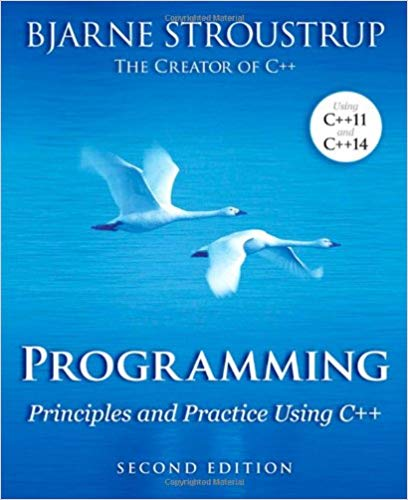
\includegraphics[width=0.23\textwidth]{Stroustrup_PPP.jpg}};
    \begin{itemize}[<+->]
        \item compiler-time errors
        \begin{itemize}[<+->]
            \item syntax errors
            \item type errors
            \item non-errors\onslide<+-> \qquad$\longrightarrow$ As you gain experience, you’ll begin to wish that the compiler would reject more code, rather than less.
            \begin{lstlisting}[]
int area(int length, int width); // calculate area of a rectangle

int x = area(10, -7); // OK: but a rectangle with a negative width?
int y = area(10.7, 9.3); // OK: but calls area(10, 9)
char z = area(100, 9999); // OK: but truncates the result
            \end{lstlisting}
        \end{itemize}
        \item link-time errors
    \end{itemize}
\end{frame}

\begin{frame}
    \frametitle{C++ build process}
    \begin{figure}
        \begin{tikzpicture}
            \node[rectangle, draw, minimum width=10em, minimum height=5ex, rounded corners, fill=Apricot] (hwcpp) at (3,0) {helloworld.cpp};
            \node[rectangle, draw, minimum width=10em, minimum height=5ex, rounded corners, fill=Yellow] (hwobj) at (0,3) {helloworld.o};
            \node[rectangle, draw, minimum width=10em, minimum height=5ex, rounded corners, fill=Yellow] (libobj) at (6,3) {externallib.o};
            \node[rectangle, draw, minimum width=10em, minimum height=5ex, rounded corners, fill=GreenYellow] (exec) at (3,6) {a.out};
            \draw[-{Latex[length=1em]}, bend left] (hwcpp) to node[midway, left] {compile} (hwobj);
            \draw[-{Latex[length=1em]}, bend right] (hwobj) to node[midway, right] {link} (exec);
            \draw[-{Latex[length=1em]}, bend left] (libobj) to (exec);
        \end{tikzpicture}
    \end{figure}
\end{frame}

\subsection<beamer:0>{Run-time errors}

\begin{frame}<beamer:0>
    \frametitle{Run-time errors}
    \tikz[overlay]\node[rotate=-6] at (60ex,5ex) {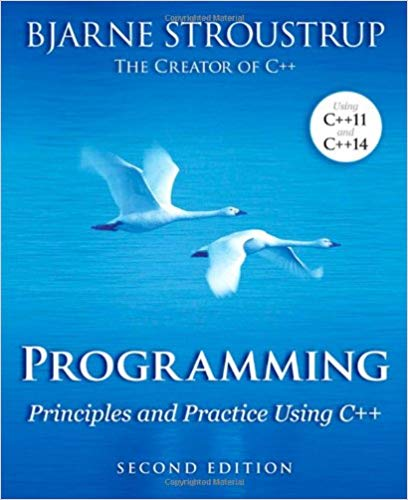
\includegraphics[width=0.23\textwidth]{Stroustrup_PPP.jpg}};
    \begin{itemize}[<+->]
        \item run-time errors
        \begin{itemize}[<+->]
            \item integration errors
            \item error reporting
            \item range errors
            \item bad inputs
            \item narrowing errors
            \item memory access errors
        \end{itemize}
    \end{itemize}
\end{frame}

\begin{frame}<beamer:0>
    \frametitle{Integration errors}
    \tikz[overlay]\node[rotate=-6] at (60ex,0ex) {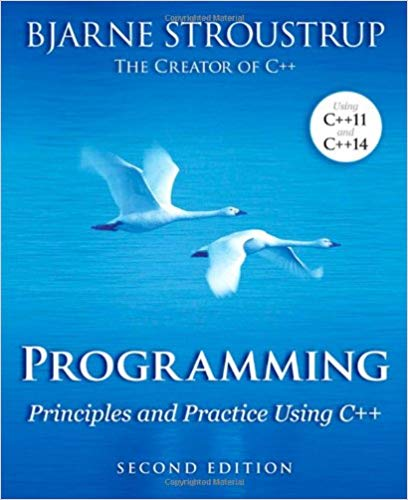
\includegraphics[width=0.23\textwidth]{Stroustrup_PPP.jpg}};
    Who should deal with errors in function calls?
    \onslide<+->
    \begin{itemize}[<+->]
        \item caller
            \begin{itemize}[<+->]
                \item code duplication
                \item are all calls error-checked?
            \end{itemize}
        \item callee
            \begin{itemize}[<+->]
                \item we can’t modify the function definition (e.g. library functions)
                \item it doesn’t know what to do in case of error
                \item it doesn’t know where it was called from
                \item performance
            \end{itemize}
    \end{itemize}
    \onslide<+->So\dots\\
    \onslide<+->Check your arguments in a function unless you have a good reason not to.
\end{frame}

\begin{frame}<beamer:0>
    \frametitle{Error reporting}
    \begin{itemize}[<+->]
        \item \texttt{cerr} \& \texttt{stderr} \onslide<+-> $\longrightarrow$ redirection: \texttt{./a.out 2> err.txt}
        \item return value
        \begin{itemize}[<+->]
            \item special values
            \item \texttt{read}, \texttt{write}, \texttt{listen} (\texttt{-1}, in combination with \texttt{errno})
            \item C++ \texttt{main} function \onslide<+-> $\longrightarrow$ \texttt{0}\onslide<+->, \texttt{cstdlib} \texttt{EXIT\_SUCCESS} \& \texttt{EXIT\_FAILURE}
            \item \texttt{exit()} (\texttt{cstdlib})
        \end{itemize}
        \item flag
        \begin{itemize}[<+->]
            \item \texttt{errno} (\texttt{errno.h})\onslide<+->, \texttt{perror} (\texttt{stdio.h})\onslide<+->, \texttt{strerror} (\texttt{string.h})
            \item \texttt{stream} error state flags\onslide<+->: \texttt{good()}\onslide<+->, \texttt{eof()}\onslide<+->, \texttt{fail()}\onslide<+->, \texttt{bad()}
        \end{itemize}
        \item exceptions
        \begin{itemize}[<+->]
            \item \texttt{throw} \& \texttt{catch}
            \item whoever could handle the error should catch the exception
            \item rethrow\onslide<+->: open files\onslide<+->, dynamically allocated memory cells
            \item \texttt{cstdexcept}
            \item not to throw exception in destructors
            \item inheritance \& subtyping
        \end{itemize}
    \end{itemize}
\end{frame}

\subsection<beamer:0>{Logic errors}

\begin{frame}<beamer:0>
    \frametitle{Logic errors}
    \tikz[overlay]\node[rotate=-6] at (60ex,4ex) {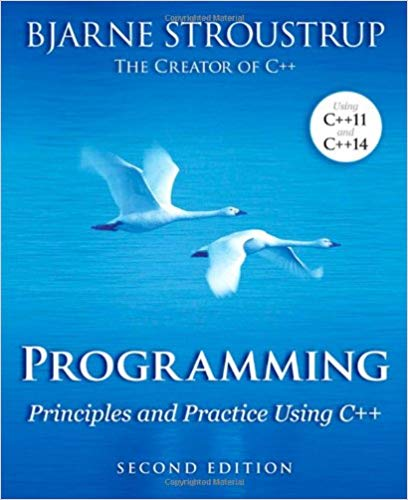
\includegraphics[width=0.23\textwidth]{Stroustrup_PPP.jpg}};
    \begin{itemize}[<+->]
        \item the most difficult to find and eliminate
        \item sources:
        \begin{itemize}[<+->]
            \item your understanding of the underlying program logic is flawed
            \item you didn’t write what you thought you wrote
            \item you made some silly error
        \end{itemize}
        \item estimation
        \begin{itemize}[<+->]
            \item Is this answer to this particular problem plausible?
            \item How would I recognize a plausible result?
        \end{itemize}
    \end{itemize}
\end{frame}

